\chapter{Shila - Implementation}
\label{chap:ShilaImplementation}

In this chapter, we present a more detailed treatise of the implementation of Shila. It builds on the explanations given in Chapter \ref{chap:ShilaIntroduction}, to read it first is therefore recommended. First, an introduction of important terms and concepts is given followed by the description of the underlying implementation structure. Then we treat the three parts of functionality (setup, connection establishment and the normal operation) for a second time, but more detailed than in Chapter \ref{chap:ShilaIntroduction} and with reference to the structure.

\section{Core Concepts and Terms}

Some important concepts and terms are explained below. These are important for further understanding of this chapter. Figure \ref{fig:IllustrationShilaPacket} summarizes them in an illustration.

\subsection{Flows}
\label{subsec:ShilaImplementationImportantConceptsFlows}

The implementation of Shila knows two types of so-called flows; the TCP-Flow and the Net-Flow.  These flows are used to uniquely identify connections and enable internal mapping tasks.

\subsubsection*{TCP-Flow}

The TCP-Flow consists of two TCP addresses representing the connection between two TCP endpoints. One of the two addresses is identified to be the source, the other to be the destination of the TCP-Flow. If used to identify a connection within an endpoint itself, then this endpoint is always the source of the TCP-Flow. Within data that is exchanged from one endpoint (source) to another (destination), the assignment is accordingly.

\subsubsection*{Net-Flow}

The Net-Flow consists of two SCION addresses that represent the connection between two SCION endpoints. The same principles apply here as for the TCP-Flow presented above. In addition to the source and destination, the Net-Flow also contains the SCION path of the corresponding connection.

\subsection{Shila-Endpoint}

A Shila endpoint is a point of contact between Shila and the outside world through which data is received or sent. The different types of these endpoints will be presented in the course of this chapter. To avoid confusion with the naming, the hierarchy of the individual endpoints is listed below.
\\
\dirtree{%
	.1 Shila-Endpoint.
	.2 Kernel-Endpoint.
	.2 Network-Endpoint.
	.3 Client-Endpoint.
	.4 Contact-Client-Endpoint.
	.4 Traffic-Client-Endpoint.
	.3 Server-Endpoint.
	.4 Contact-Server-Endpoint.
	.4 Traffic-Server-Endpoint.
}

\subsection{Shila-Packet}

For the exchange of data so-called Shila-Packets are used. A packet contains the actual payload, namely the IP datagram exchanged between two TCP endpoints. It furthermore holds a link to its creating Shila-Endpoint and is associated with a TCP-Flow as well as Net-Flow. 

\begin{figure}[H]
	\begin{center}
		\def\svgwidth{1\textwidth}
		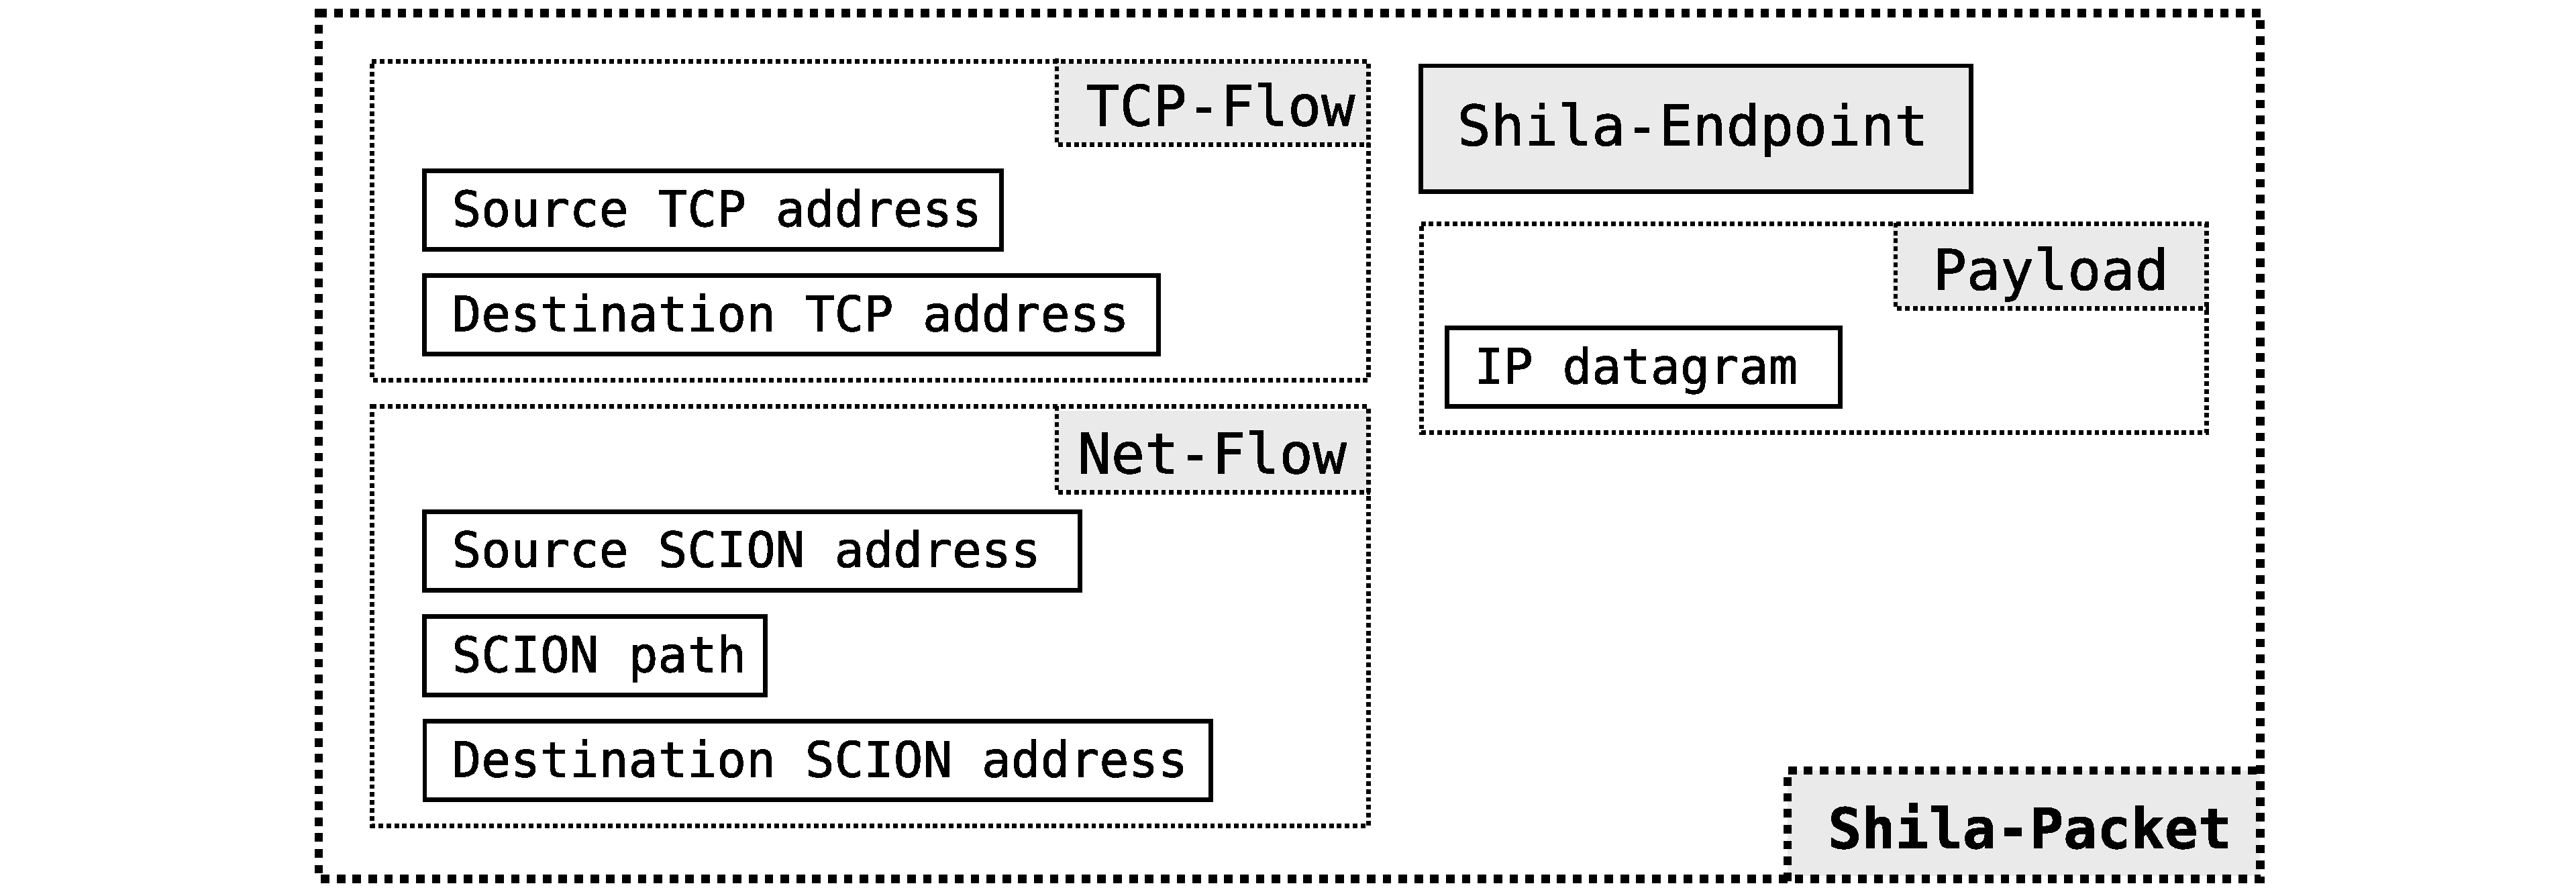
\includegraphics[scale=0.2]{../illustrations/implementation/ShilaPacket.pdf}   
		\caption[Caption for the list of figures.]{Illustration of the Shila-Packet containing the payload, a handle to its creating Shila-Endpoint and the associated TCP-Flow and Net-Flow.}
		\label{fig:IllustrationShilaPacket}
	\end{center}
\end{figure}

\newpage
\section{Structure}
\label{sec:ImplementationStructure}

In the outermost level, the implementation of Shila can be divided into five different parts, illustrated in Figure \ref{fig:ImplementationModulesOutermost}. The Kernel-Side handles the creation of and the interaction with the virtual interfaces and handles the data exchange with the TCP applications. The Network-Side is responsible for the creation and handling of backbone connections over SCION and the data exchange with Shila instances on other computers. The Working-Side in between receives incoming data from both sides and makes sure that it is handed over to the correct Shila-Connection. The Shila-Connection itself maintains the state of a connection and delivers the data to the desired destination. To be able to do this, the Shila-Connection relies on the services of the Router.  The data exchange between the individual parts takes place via traffic channels, transporting the Shila-Packets. In the following, we discuss each of the parts in more detail and provide a more detailed subdivision of the structure into further subparts and their functionality.  

\begin{figure}[H]
	\begin{center}
		\def\svgwidth{1\textwidth}
		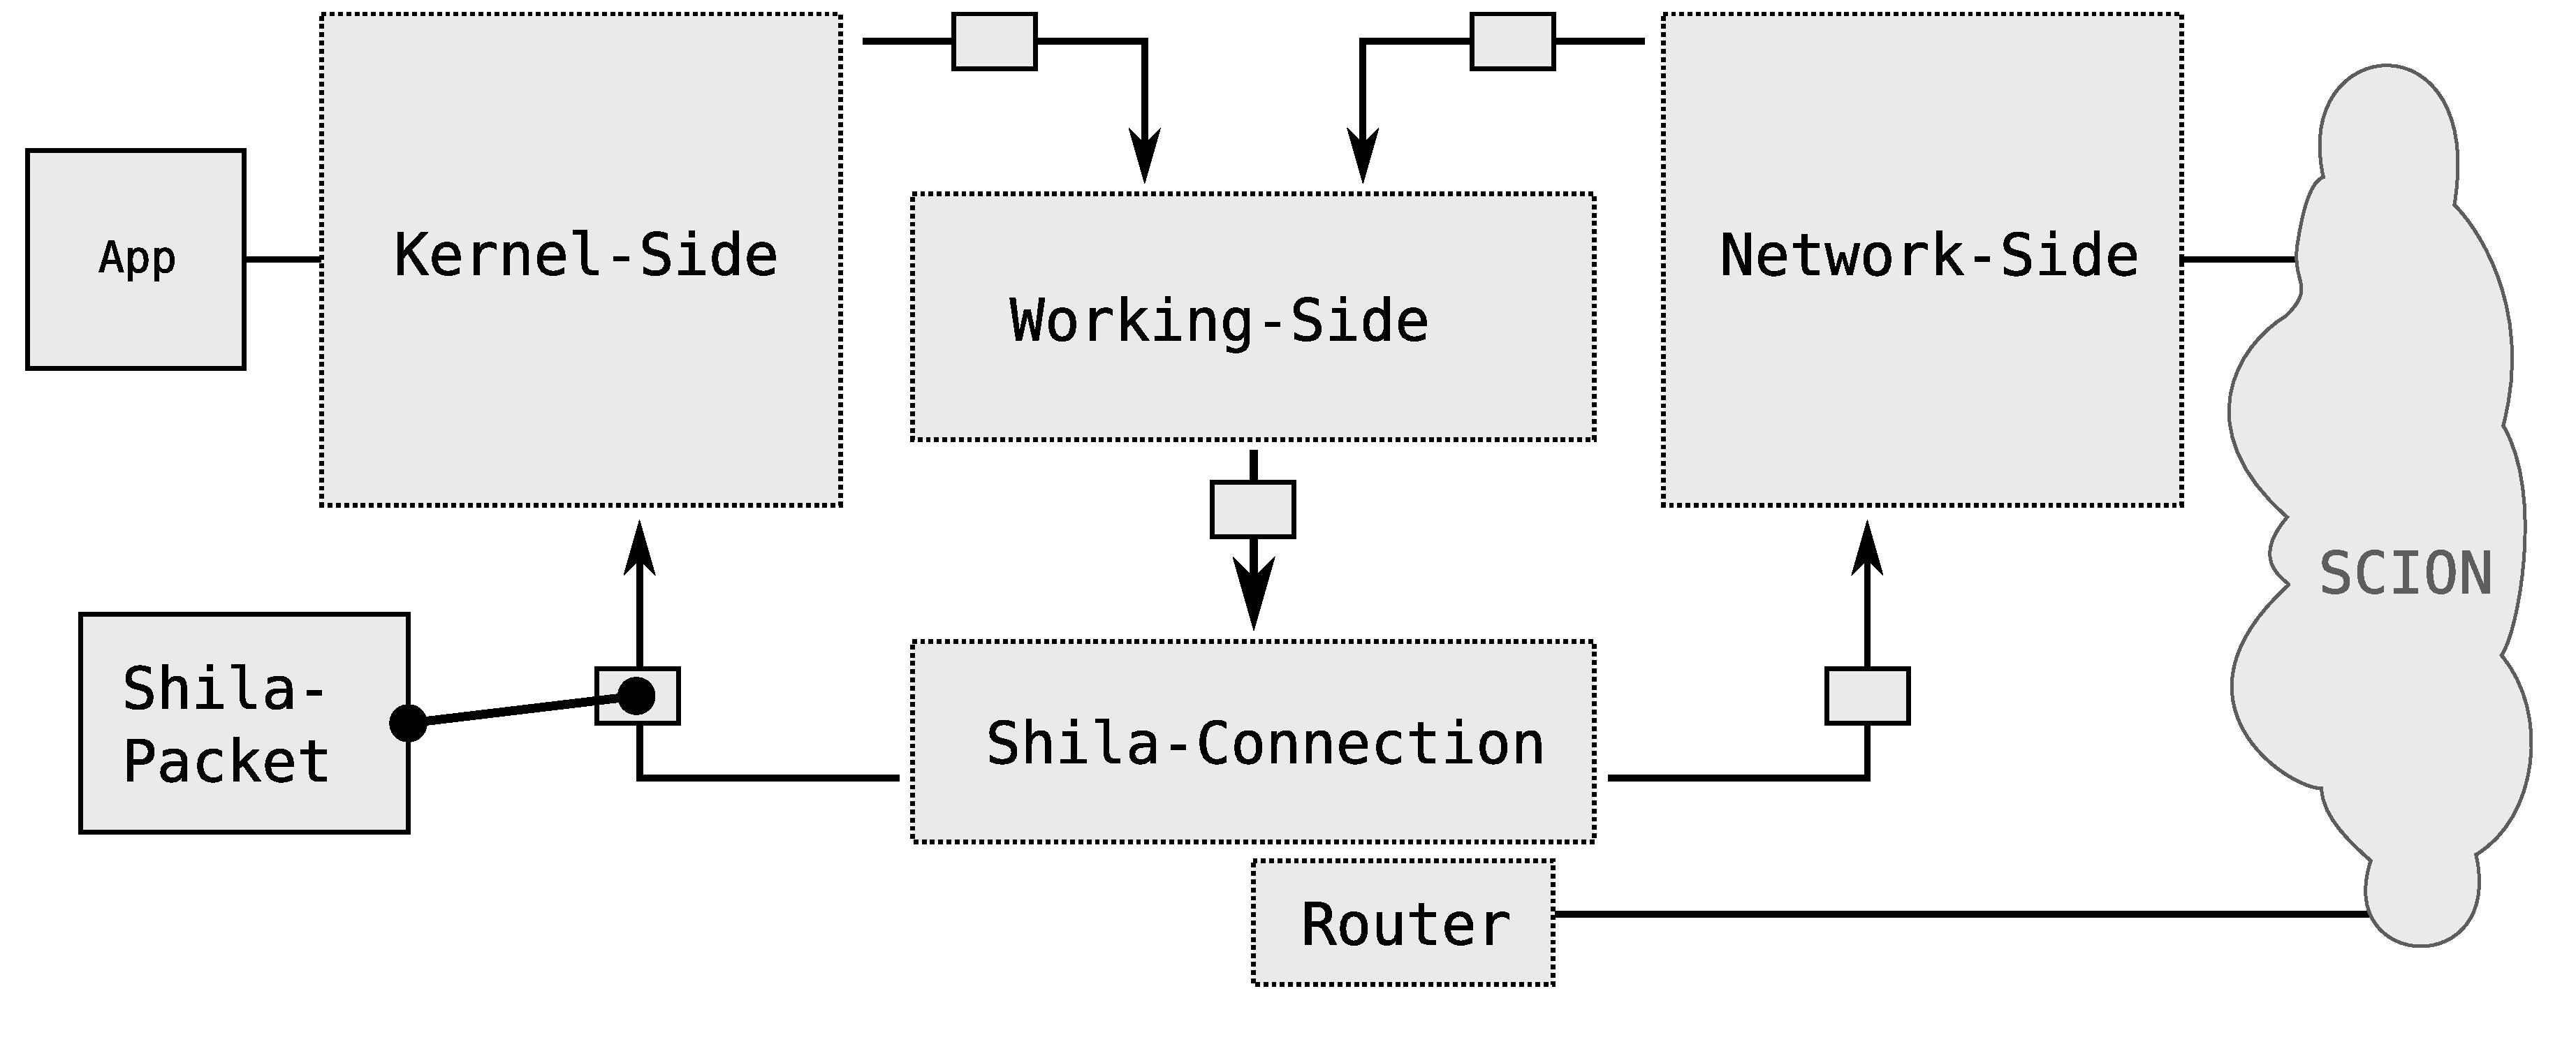
\includegraphics[scale=0.2]{../illustrations/implementation/ModulesOutermost.pdf}   
		\caption[Caption for the list of figures.]{Illustration of the outermost division of the implementation into different parts.}
		\label{fig:ImplementationModulesOutermost}
	\end{center}
\end{figure}

\subsection{Kernel-Side}

The Kernel-Side, shown in Figure \ref{fig:ImplementationModulesKernelSide}, is managed by an appropriate manager, allocating the network namespaces and creating the individual Kernel-Endpoints, which are located within the namespaces. It furthermore provides an interface for the creation of Kernel-Endpoints and it allows to query for the traffic channels held by these endpoints. The Kernel-Endpoint-Mapping stores a mapping from IP addresses to the corresponding Kernel-Endpoints.  

\begin{figure}
	\begin{center}
		\def\svgwidth{1\textwidth}
		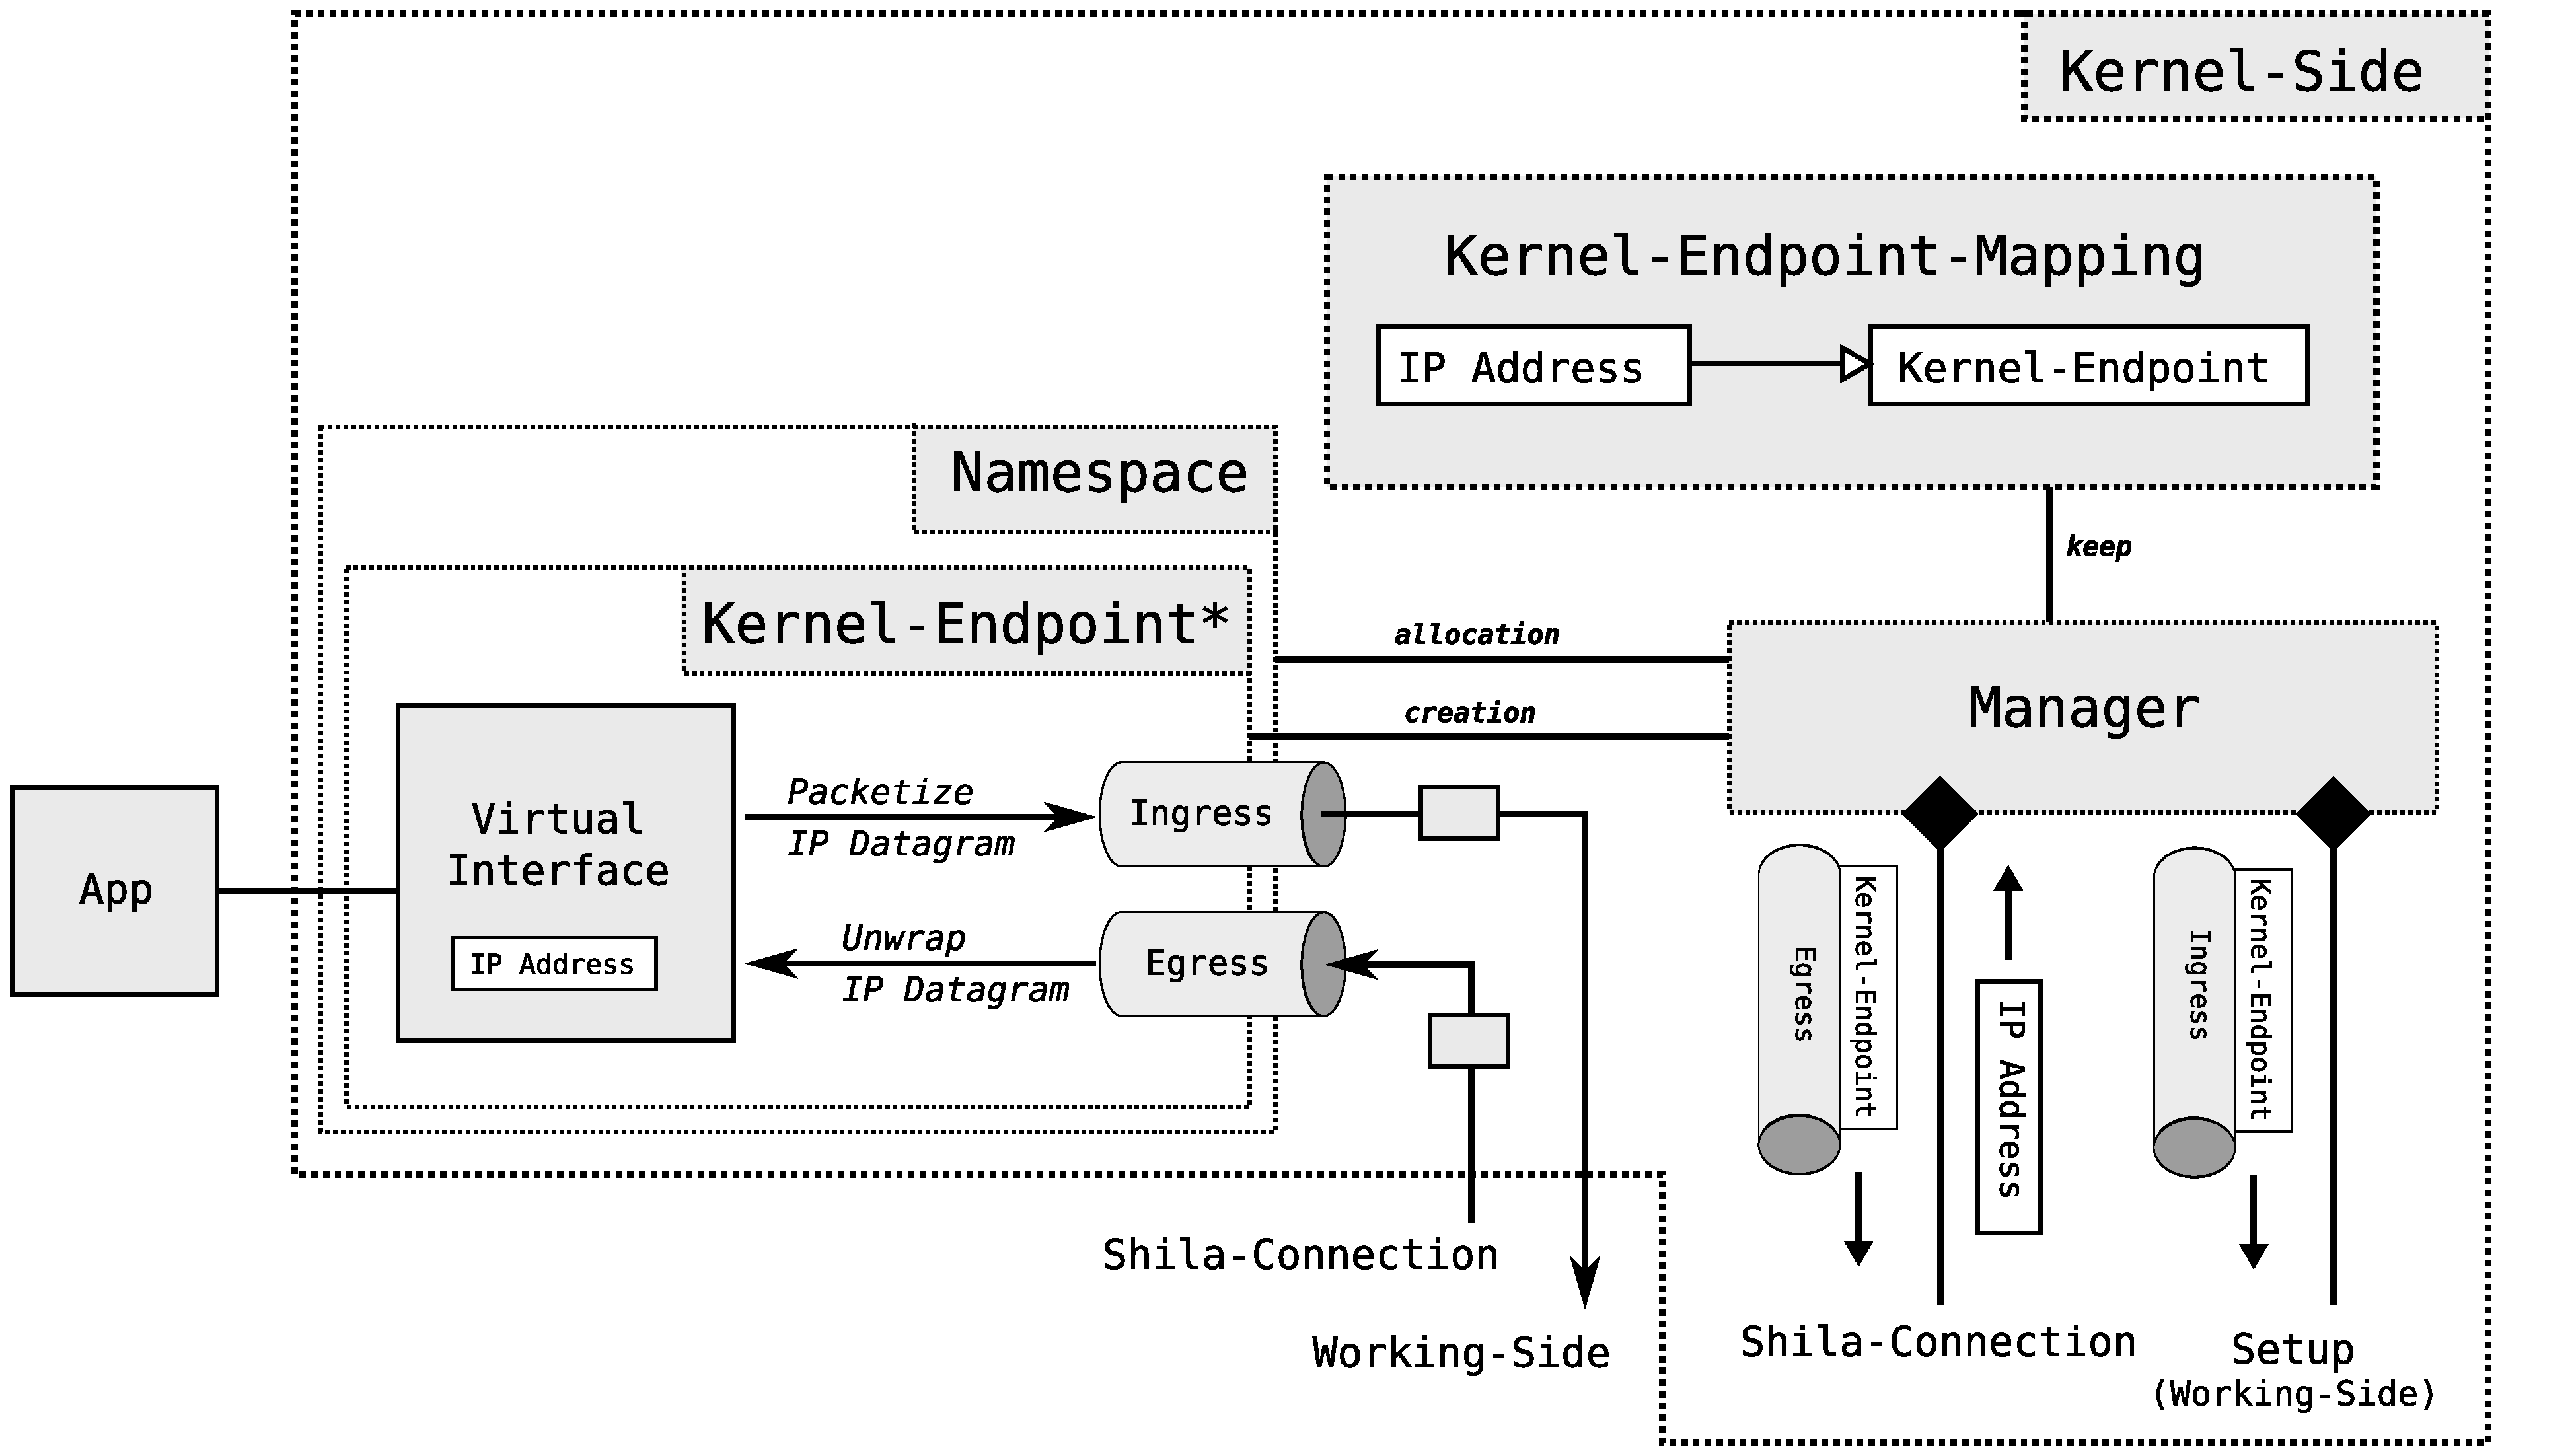
\includegraphics[scale=0.2]{../illustrations/implementation/ModulesKernelSide.pdf}   
		\caption[Caption for the list of figures.]{Illustration of the Kernel-Side with its subparts.}
		\label{fig:ImplementationModulesKernelSide}
	\end{center}
\end{figure}


\subsubsection{Kernel-Endpoint}

The Kernel-Endpoint creates and holds the virtual network interface over which the data exchange with the TCP endpoints takes place. Every Kernel-Endpoint is identified by an IP address, namely the IP address assigned to its underlying virtual interface. It also holds two traffic channels. For an IP frame received through the virtual interface, the TCP-Flow is determined and a newly created Shila-Packet is sent via the ingress channel to the working side. Through the egress channel packets from Shila-Connections are received. From these packets, the payload is taken and transferred to the virtual interface and from there to the TCP endpoint.

\subsubsection{Virtual Interface}

Shila uses the Universal TUN/TAP device driver \cite{TUNTAPDriver} to set up virtual network devices on the host. Such a virtual network device is perceived by the kernel as a real Ethernet device. The difference is that traffic from the kernel is not sent through a physical medium but can be read by an application, in our case Shila. On the other hand, the virtual device does not receive the data over the cable but from an application, again Shila.

Each virtual network interface has an IP address assigned to it. When a TCP endpoint sends data over a virtual device, Shila receives the corresponding IP datagrams. Each of these contains a TCP flow. The source TCP address consists of the IP address of the virtual device and an arbitrary port. The destination address is the TCP address the application wants to send data to. Conversely; when Shila writes payload, an IP datagram, to a virtual device, then the kernel forwards it to the application identified by the destination TCP address.  

\subsection{Network-Side}

The Network-Side is also orchestrated by an appropriate manager. At startup, the manager takes care of establishing the Contact-Server-Endpoint. It furthermore provides the interface to Shila-Connections for the creation of new Contact-Client-Endpoints, Traffic-Client-Endpoints and Traffic-Server-Endpoints. The Network-Side holds three different mappings. Two to get the corresponding Client-Endpoint for a given TCP-Flow, and one to get the Server-Endpoint associated with the SCION source address. These mappings are only used by the manager to interact with the endpoints, e.g. for the deallocation in case of a disconnection. They are not needed for the data exchange itself. After establishing the connection, the corresponding entities directly hold a handle of the traffic channels from the respective endpoints. Figure \ref{fig:ImplementationModulesNetworkSide} illustrates these Network-Endpoint-Mappings as part of the whole kernel side and its subparts.  

\subsubsection{Server-Endpoint}

The Server-Endpoint is one of two types of Shila-Endpoints found on the Network-Side. It can be further divided into Contact-Server-Endpoint and Traffic-Server-Endpoint. However, there is no difference in basic functionality between the two. We mention the differences in the discussion of setup¨ and connection establishment, see Section \ref{sec:ImplementationSetup} and Section \ref{sec:ImplementationConnectionEstablishment}.

A Server-Endpoint holds and handles a collection of Backbone-Connections, i.e. connections through the SCION network to Client-Endpoints running on other instances of Shila. Each such Backbone-Connection is associated with a Net-Flow. The Server-Endpoint-Mapping\footnote{In Figure \ref{fig:ImplementationModulesNetworkSide}, this mapping is shown as part of the Network-Endpoint-Mappings.} in the Network-Side uses the source address of this Net-Flow as a key. Inside the endpoint, the corresponding destination address is used as the key for the Backbone-Connection-Mapping. %Note that this mapping is used in the actual data exchange. 

A Backbone-Connection itself uses the appnet package \cite{Appnet} to establish the connection in SCION. Data received from the SCION network is packed into a Shila packet by the responsible backbone connection and sent via the ingress traffic channel of the server to the Working-Side. Packets received from Shila-Connections are allocated to their Backbone-Connection using their Net-Flow and the Backbone-Connection-Mapping. From there, the payload is sent to the SCION network.

\subsubsection{Client-Endpoint}

The Client-Endpoint is the other type of Shila-Endpoints within the Network-Side. It is the initiating party of a Backbone-Connection and is associated with just a single Net-Flow. As with the Server-Endpoint, a distinction is made between a Contact-Client-Endpoint and a Traffic-Client-Endpoint, again discussed later. The data exchange between the SCION network and the internal Shila units works via the appnet package and two traffic channels. Since only one Backbone-Connection is assigned to a single Client-Endpoint, no mapping is required inside the endpoint.

\begin{figure}
	\begin{center}
		\def\svgwidth{1\textwidth}
		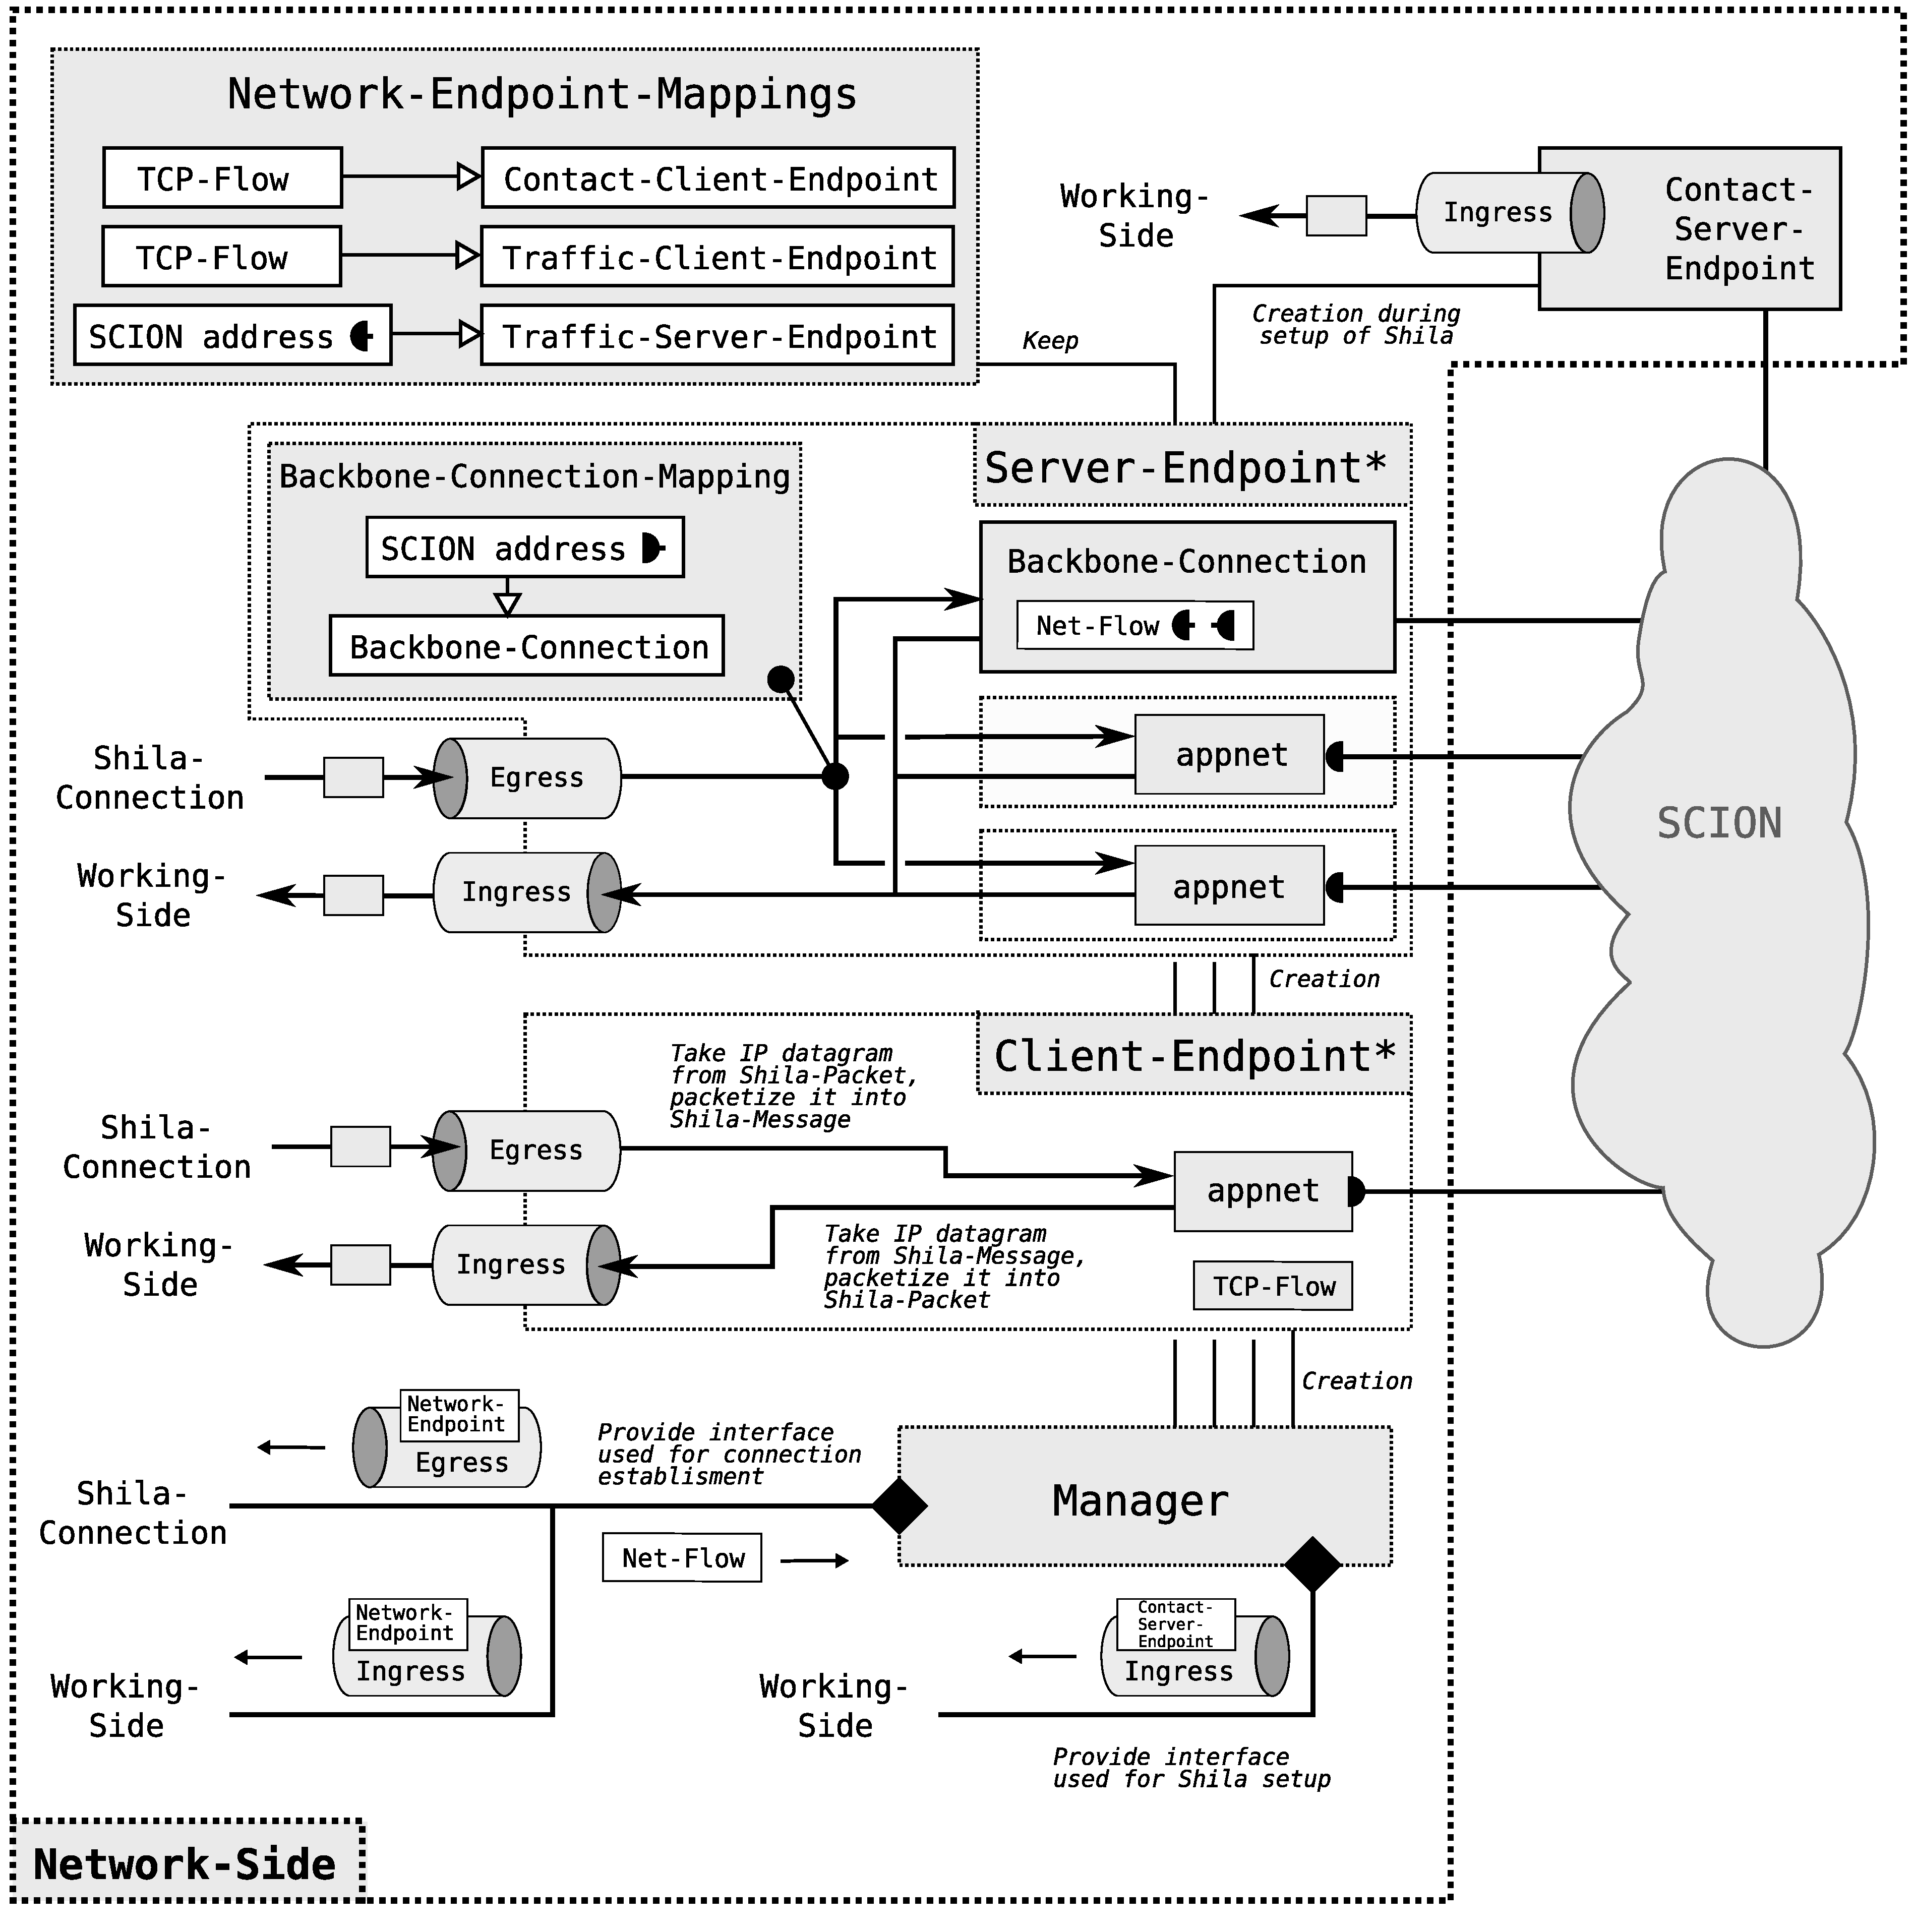
\includegraphics[scale=0.2]{../illustrations/implementation/ModulesNetworkSide.pdf}   
		\caption[Caption for the list of figures.]{Illustration of the Network-Side with its subparts.}
		\label{fig:ImplementationModulesNetworkSide}
	\end{center}
\end{figure}

\subsection{Working-Side}

Upon the arrival of a Shila-Packet at the Working-Side it is processed by a dedicated worker. Its TCP-Flow is extracted and used as the key for the Shila-Connection-Mapping, the heart of the Working-Side. It contains the mapping from TCP-Flows to Shila-Connections. If there is no corresponding entry available then a new Shila-Connection is created and inserted into the mapping. Once obtained, the responsible worker processes the Shila-Packet through the associated Shila-Connection. The described process is illustrated in Figure \ref{fig:ImplementationProcessWorkingSide}.

\begin{figure}[H]
	\begin{center}
		\def\svgwidth{1\textwidth}
		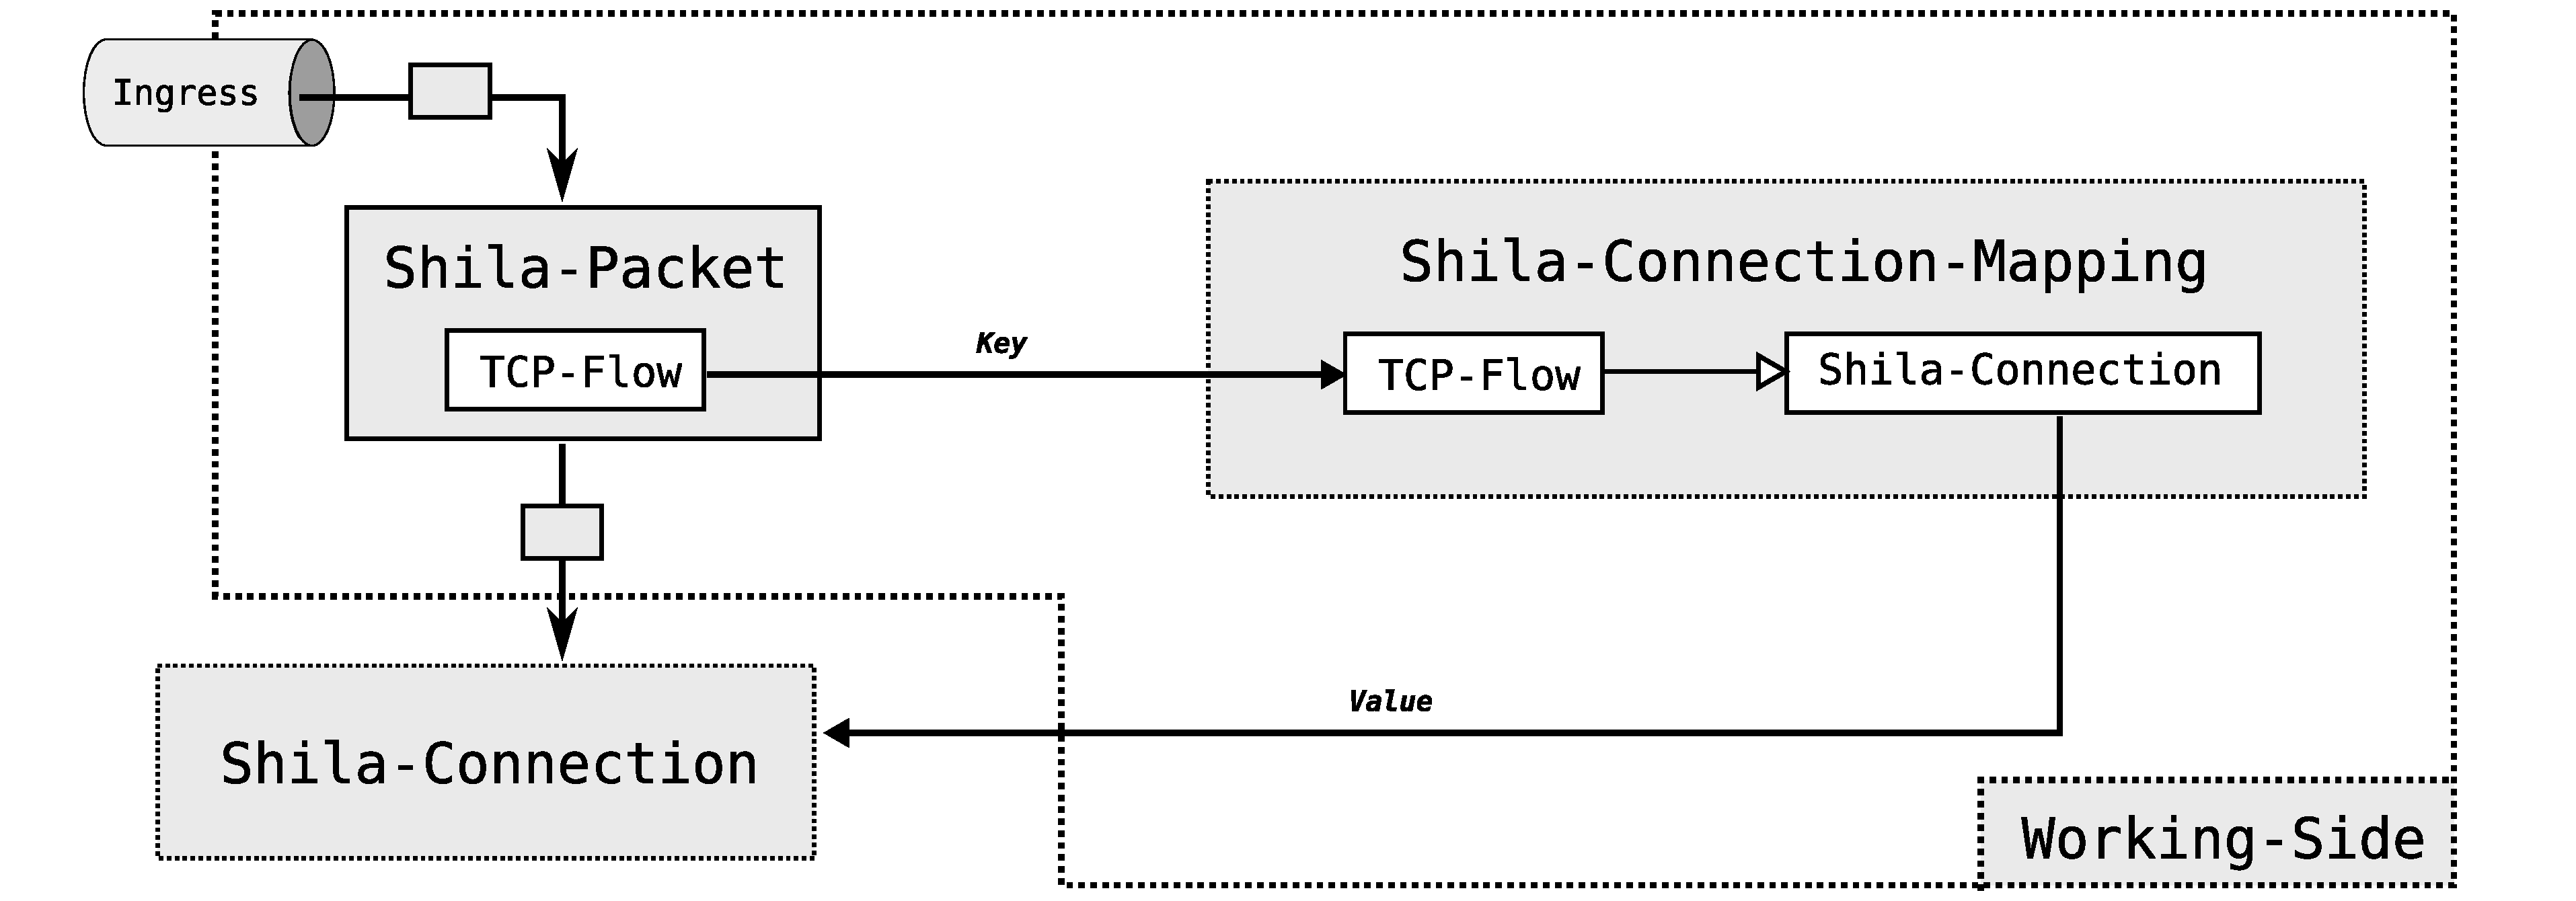
\includegraphics[scale=0.2]{../illustrations/implementation/ProcessWorkingSide.pdf}   
		\caption[Caption for the list of figures.]{Illustration of the Working-Side.}
		\label{fig:ImplementationProcessWorkingSide}
	\end{center}
\end{figure}

\subsection{Shila-Connection}

The Shila-Connection, depicted in Figure \ref{fig:ImplementationShilaConnection}, is the main part of Shila, with its logic responsible for establishing and maintaining connections. The centerpiece is the state machine and the close coupling to the router, which provides SCION destination and path information. During connection establishment, the Shila-Connection uses the interfaces of Kernel-Side and Network-Side as well as the functionalities provided by the Router to put its traffic channels into place. Once established, the packages flow smoothly through the Shila-Connection to their respective destination endpoints without much interaction. Every Shila-Connection is identified by its TCP-Flow and holds, once the connection is established, the corresponding Net-Flow.

\begin{figure}
	\begin{center}
		\def\svgwidth{1\textwidth}
		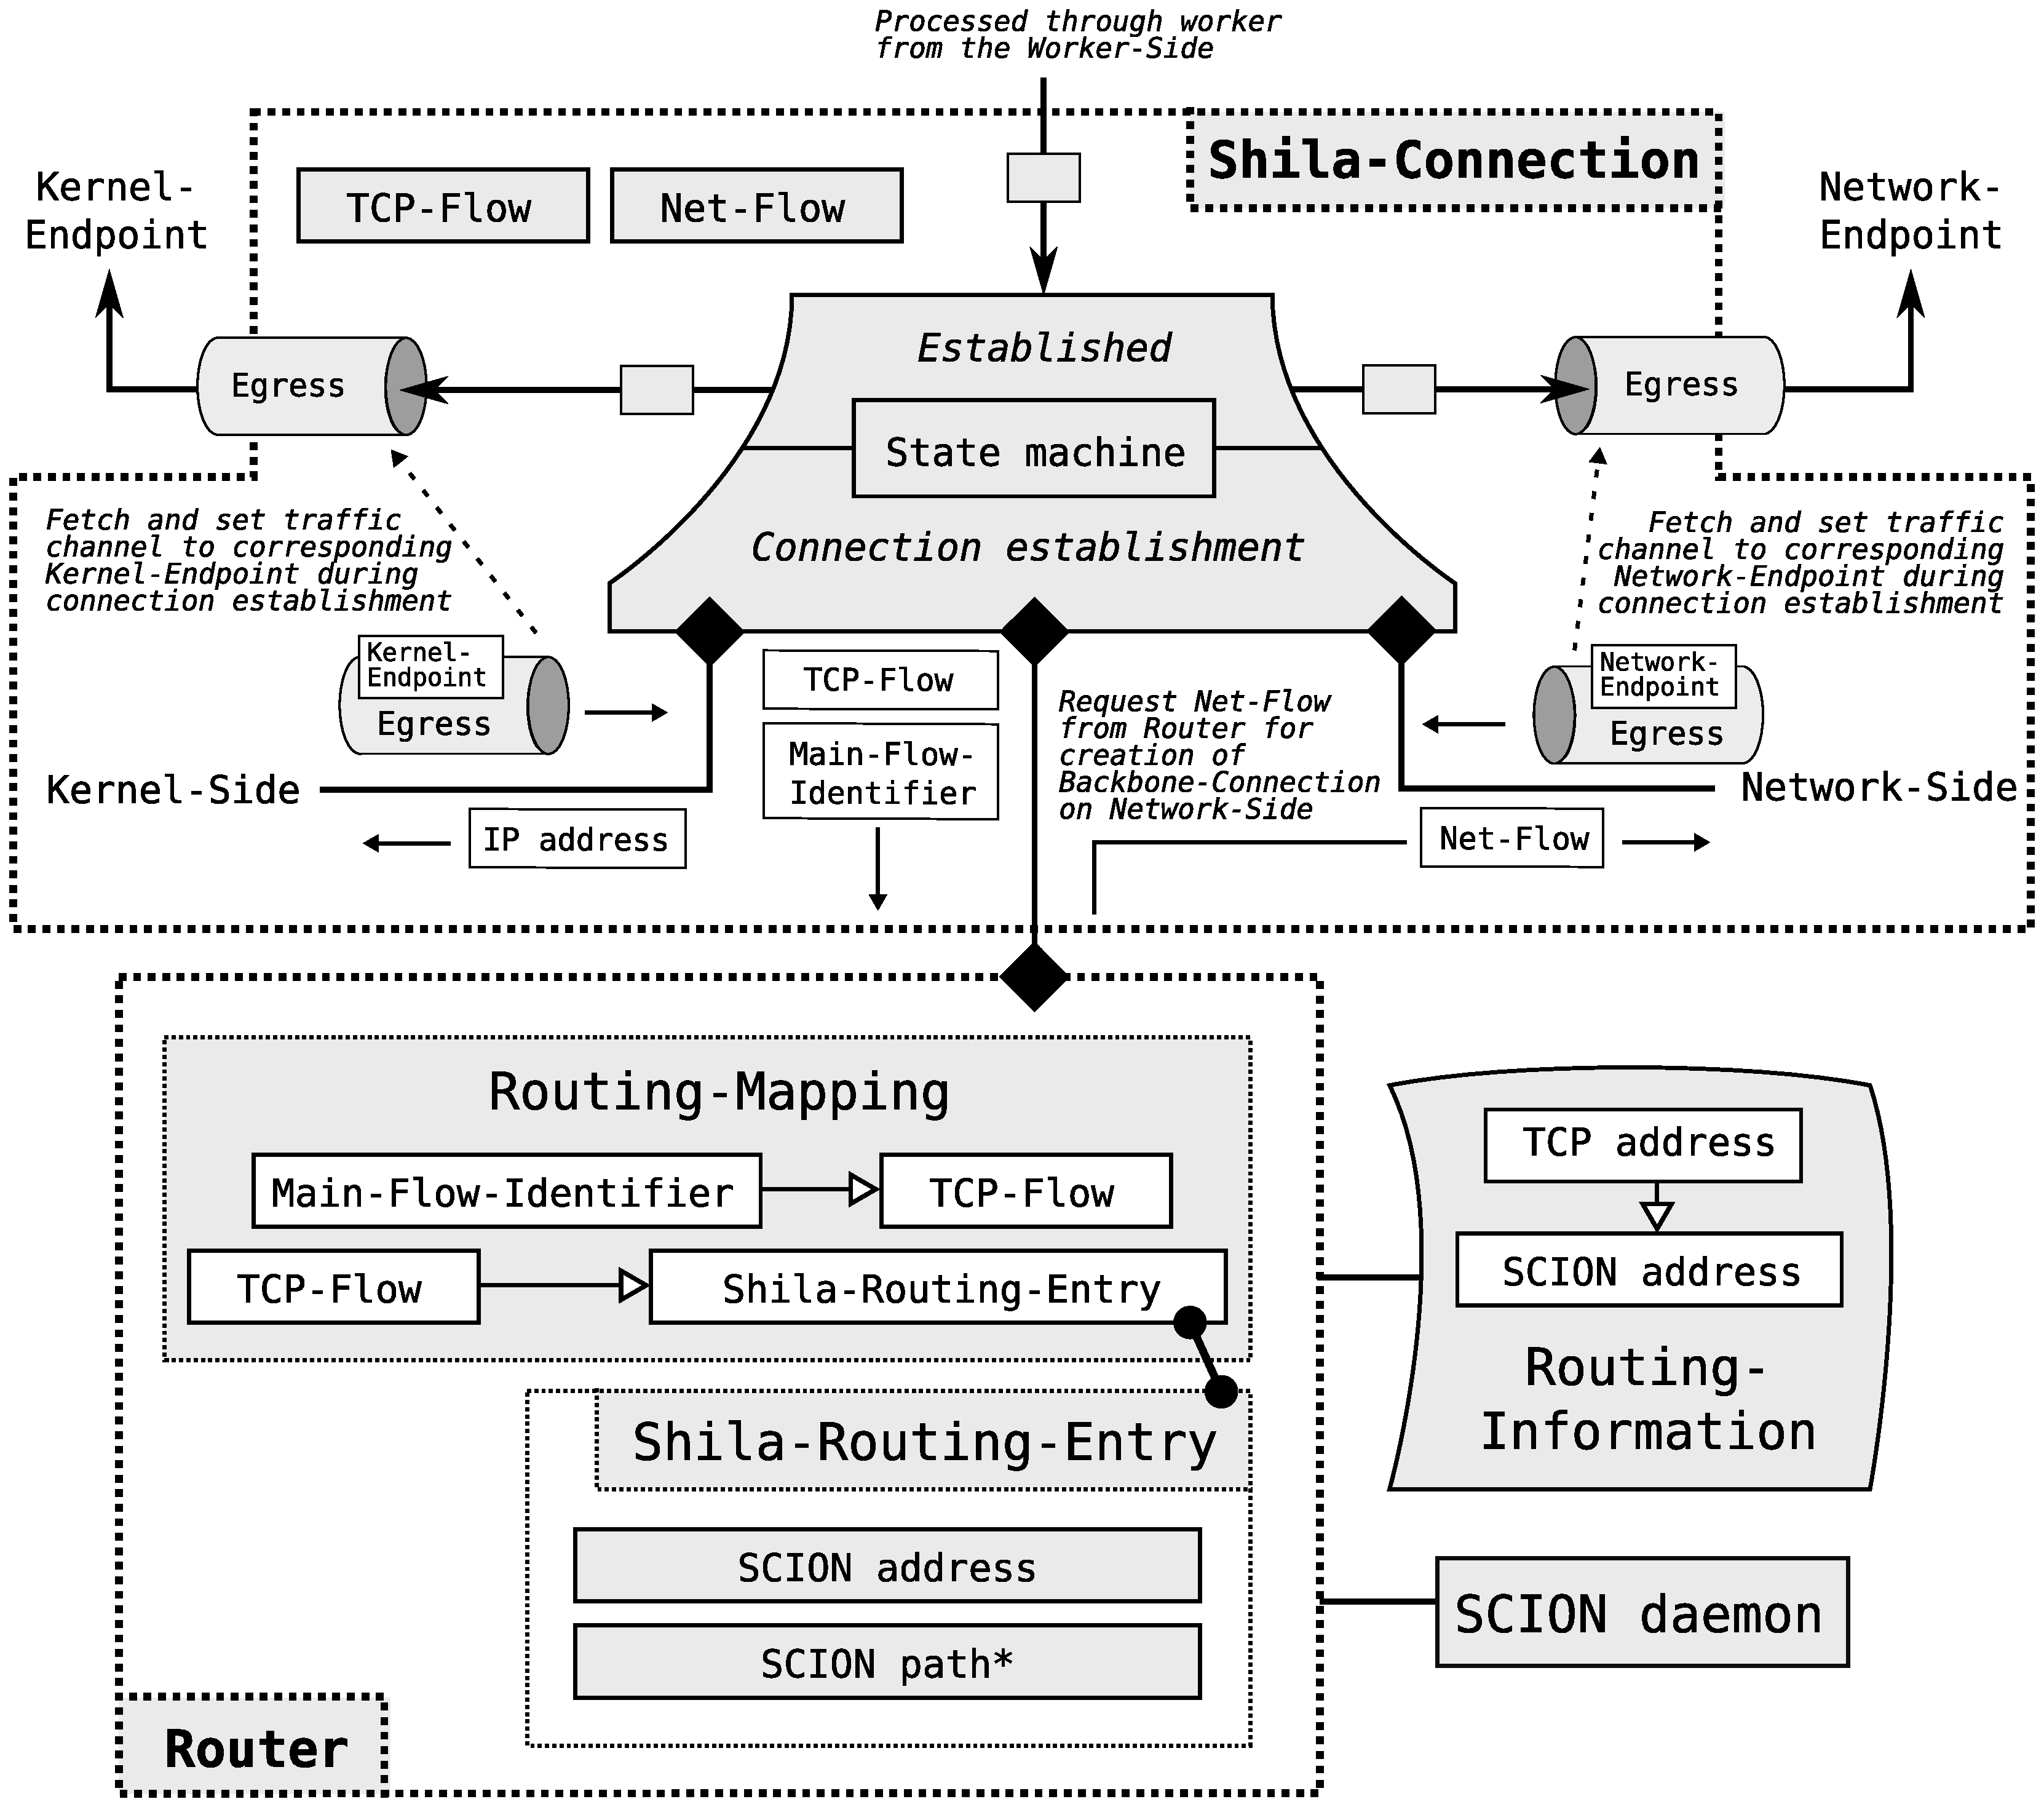
\includegraphics[scale=0.2]{../illustrations/implementation/PartsShilaConnection.pdf}   
		\caption[Caption for the list of figures.]{Illustration of the Shila-Connection together with the Router. The Shila-Connection receives the packets assigned to it through the Working-Side. If the connection is already established, the packet is forwarded directly to its destination via the egress traffic channel. During the connection setup, the Shila-Connection first uses the Router to determine the Net-Flow and then requests the egress traffic channels from the Kernel-Side and Network-Side.}
		\label{fig:ImplementationShilaConnection}
	\end{center}
\end{figure}

\subsection{Router}
\label{sec:ImplementationRouter}

The Router supplies the Shila-Connection with the Net-Flow as part of the connection establishment. It is connected to the SCION daemon running on the host and has access to a hardcoded mapping between TCP and SCION addresses. This mapping is denoted as Routing-Information. The Router illustrated as part of Figure \ref{fig:ImplementationShilaConnection} also maintains a Routing-Mapping which uses TCP-Flow as a key to store Shila-Routing-Entries and an additional mapping from Main-Flow-Identifier to TCP-Flows.

\subsubsection{Shila-Routing-Entry}

A Shila-Routing-Entry stores a SCION address and several paths leading through the SCION network to this destination. The number of stored paths depends on the setting of Shila, namely on the number of virtual interfaces created in the egress namespace. Also stored for each of the paths is its quality, given in different metrics. These metrics are used as a decision criterion in the process of path selection which is itself part of the creation of routing entries. The whole process of the routing, i.e. the creation of these entries as well as the procedure of path selection is described in its own Section \ref{sec:ImplementationPathSelection}.

\newpage
\section{Setup}
\label{sec:ImplementationSetup}

In this section, we describe the crucial steps executed during the setup of Shila. The description is similar to the one given in the Introduction to Shila. This time its more detailed and also refers to the structure presented in the sections and illustrations above.

\paragraph{Loading of the Routing-Information}

To perform its function of providing translations between a TCP-Flow and a Net-Flow, the Router establishes a connection to the SCION daemon and loads the Routing-Information from disk. Saved as a JSON file it contains the translation from a TCP to a SCION address. Currently, there is no other way to provide the Router with this necessary information. However, alternatives are certainly conceivable and are mentioned in the concluding Chapter \ref{chap:FutureWork}.

\paragraph{Setup of Namespaces}

The manager on the kernel side creates the two network namespaces \cite{LinuxNetworkNamespacesUbuntuManual,LinuxNetworkNamespacesIntroduction}, the ingress and the egress namespace, in a first step. System resources, like network devices or IP routing tables, associated with networking and assigned to different namespaces are isolated from each other. This simplifies the development and setup of the kernel side but on the downside requires the TCP applications to be started within the corresponding namespaces. For further discussions with regard to namespaces see Chapter \ref{chap:FutureWork}.

\paragraph{Creation of Kernel-Endpoints hosting virtual Interfaces}

In the second step, the manager creates the Kernel-Endpoints in the appropriate namespaces. In the ingress namespace, this is exactly one, in the egress namespace, this is a number selected by the user between one and a maximum of eight. The number of Kernel-Endpoints selected in the egress namespace later corresponds to the number of paths used for a connection. The current implementation of MPTCP supports up to eight interfaces. Having Shila to support more is therefore useless, but can be realized without problems if necessary in the future.

Each Kernel-Endpoint contains a virtual interface to which an IP address is assigned. This address is also assigned to the Kernel-Endpoint itself and is used as a key in the Kernel-Endpoint-Mapping. The virtual interface in the ingress namespace is assigned a default address (10.7.0.9), the assignment in the egress namespace is done at random. Upon its establishment, every Kernel-Endpoint creates two traffic channels. The ingress channel, which is used for forwarding incoming data, is registered at the working side. 

\paragraph{Contact-Server-Endpoint}

During the setup, the manager in the Network-Site creates just one Network-Endpoint; the Contact-Server-Endpoint. This endpoint starts listening for incoming Backbone-Connections on the default SCION port 7654 using the appnet package. In contrast to all other Shila-Endpoints, it needs only one traffic channel, namely for incoming messages that initiate the establishment of a new connection. This channel is registered with the Working-Side.

After the successful setup, applications can be started in the respective namespaces and the data exchange is initiated with the connection establishment.

\section{Connection Establishment}
\label{sec:ImplementationConnectionEstablishment}

In this section, we again discuss the individual steps in the establishment of a new connection between two TCP endpoints. We use the explanation of Section \ref{subsec:ShilaConnectionEstablishment} as a basis, but go into more detail and extend the sequence with intermediate steps, referring to the treatise of the structure given in Section \ref{sec:ImplementationStructure}. The starting point and the example used is the same one as used in the introductory treatise of the connection establishment in Section \ref{subsec:ShilaConnectionEstablishment}. Illustration \ref{fig:ConnectionEstablishment} shows the state after the successful establishment of the connection with the values from the example discussed. These values are also mentioned in the discussion of the individual steps below. In the used notation, the source comes first and then the destination.

\subsection{Main-Flow Establishment}

We start with a more detailed discussion of the Main-Flow establishment. 

\begin{description}
	\item[M-1] On Host 2, the server instance of iPerf3 starts listening for incoming TCP connections. It, therefore, binds to the virtual interface in the Shila ingress namespace on the TCP address 10.7.0.9:27041. This step is not recognized by the Kernel-Endpoint hosting the corresponding virtual interface.
	\item[M-2] On Host 1, the client instance of iPerf3 tries to connect to its server counterpart on TCP address 10.7.0.9:27041. For the connection establishment, an IP datagram, containing the TCP-SYN, is sent via one of the virtual interfaces in the egress namespace. Let's say It is identified by the IP address 10.0.0.1 and the socket bound to port 11111.
	\item[M-3] The Kernel-Endpoint owning the corresponding virtual interface receives the IP datagram and puts it into a Shila-Packet. While payload, Shila-Endpoint and TCP-Flow$^{1}$ are determined, the Net-Flow for the created Shila-Packet is not yet known. The packet is now forwarded to the Working-Side.\medskip\\{\small[10.0.0.1:11111, 10.7.0.9:27041]$^{1}$}
	\item[M-4] The Working-Side uses the TCP-Flow, extracted from the packet, as the key into the Shila-Connection-Mapping. Since there is no corresponding Shila-Connection, a new one is created and the Shila-Packet is forwarded on to it.  
	\item[M-5] To be able to forward the received Shila-Packet, the newly created Shila-Connection has to first determine the destination SCION address and path. It does this by querying the Router, which determines the corresponding parts of the Net-Flow for the TCP-Flow of the packet.
\end{description}

The entire process of determining the Net-Flow, i.e. address translation and the path selection, is explained in the following Section \ref{sec:ImplementationPathSelection}. To include the explanation as part of this sequence, would make it unnecessary bulky to read. For the next step M-6, we assume that the required parts of the Net-Flow are determined.

\begin{description}
	\item[M-6] The Shila-Connection uses the interface of the manager on the Network-Side to initiate the creation of a Contact-Client-Endpoint. It provides the Net-Flow$^2$ it has received from the Router.\medskip\\{\small[1-ff00:0:112,127.0.0.1, 2-ff00:0:220,127.0.0.1:27041]$^2$}
	\item[M-7] The Contact-Client-Endpoint establishes the so-called Contact-Backbone-Connection to the Contact-Server-Endpoint. It uses the source address available in the provided Net-Flow together with the default SCION port of the listening server. For our example, we assume that the outgoing SCION port of the Contact-Client-Endpoint is 12121. This information completes the Net-Flow of the Contact-Backbone-Connection$^{3}$.\medskip\\{\small [1-ff00:0:112,127.0.0.1:12121, 2-ff00:0:220,127.0.0.1:7654]$^{3}$}
%\end{description}
%	
%The establishment of a Backbone-Connection between Client-Endpoint and Server-Endpoint is described separately in Section %\ref{sec:ImplementationEstOfBackboneConnections}. For the next step, \textbf{M-9}, we assume that the Backbone-Connection %between Contact-Client-Endpoint on Host 1 and Contact-Server-Endpoint on Host 2 is established.
%	
%\begin{description}
	\item[M-8] With the successful setup of the Contact-Client-Endpoint, the Shila-Connection receives the handle to its egress traffic channel. Using this channel, the Shila-Packet, and hence the initial IP datagram containing the TCP-SYN is now transferred to the Contact-Server-Endpoint running on the Shila instance on Host 2. %The Shila-Connection sets its Net-Flow$^{3}$ to be the one of the Contact-Backbone-Connection.%
	\item[M-9] The IP datagram is received at the Contact-Server-Endpoint on Host 2. There, it is put into a Shila-Packet and forwarded via the ingress traffic channel to the working side. The Net-Flow$^{4}$ (namely that of the backbone connection between Contact-Client-Endpoint and Contact-Server-Endpoint) can already be assigned to the newly created Shila-Packet. The TCP-Flow$^{5}$ is also known since it was transmitted with the establishment of the Contact-Backbone-Connection.\medskip\\{\small [2-ff00:0:220,127.0.0.1:7654, 1-ff00:0:112,127.0.0.1:12121]$^{4}$}\\{\small [10.7.0.9:27041, 10.0.0.1:11111]$^{5}$} 
	\item[M-10] The Working-Site on Host 2 cannot find a Shila-Connection for the TCP-Flow$^{5}$ in the Shila-Packet. Accordingly, a new one is created and the packet is passed to it.
	\item[M-11] Inside the Shila-Connection, three tasks are performed. First, the Net-Flow$^{4}$ of the Shila-Packet is extracted and assigned to the Shila-Connection.  Note, until now it was the Net-Flow of the associated Contact-Backbone-Connection. Second, the Shila-Packet is forwarded. The source IP address of its TCP-Flow$^{5}$ is used to retrieve the egress traffic channel from the Kernel-Endpoint residing in the ingress namespace. This is done by the Shila-Connection by querying the Kernel-Endpoint-Mapping inside the Kernel-Side. For our example, the IP address used as the key is 10.7.0.9. The Shila-Packet is forwarded through the respective channel, once it is obtained. Third, the Shila-Connection causes the creation of a Traffic-Server-Endpoint which is ready for new Backbone-Connections at SCION port 27041. The ingress traffic channel is registered with the Working-Side and the Shila connection receives a handle to respective the egress traffic channel.
	\item[M-12] The Kernel-Endpoint receives the Shila-Packet, extracts its payload and sends the IP datagram containing the TCP-SYN through the virtual interface towards the listening iPerf3 server instance.
	\item[M-13] In the meantime, the Shila connection of Host 1 has initiated the creation of a Traffic-Client-Endpoint. This now establishes a Backbone-Connection to its opposite, called a Traffic-Backbone-Connection. This time, in comparison to step M-8, using the complete Net-Flow. Let's assume that the Traffic-Client-Endpoint binds locally to SCION port 34343, completing the Net-Flow$^{6}$ of the Traffic-Backbone-Connection. This Net-Flow is assigned to Shila-Connection on Host 1.
	\medskip\\{\small [1-ff00:0:112,127.0.0.1:34343, 2-ff00:0:220,127.0.0.1:27041]$^{6}$}
	\item[M-14] With the successful establishment of the Traffic-Backbone-Connection, the involved Server-Endpoint on Host 2 receives the TCP-Flow$^{5}$ as well as two Net-Flows. The Net-Flow$^{4}$ of Contact-Backbone-Connection and the Net-Flow$^{7}$ of the Traffic-Backbone-Connection. Both of its destination addresses are used as key to store the Traffic-Backbone-Connection in Backbone-Connection-Mapping. This is required since the Shila-Connection sends back all data, including the data received via the Contact-Server-Endpoint, via the Traffic-Server-Endpoint. Remember, the Shila-Connection on Host 2 currently holds the Net-Flow of the Contact-Backbone-Connection which now can be updated to the one of the Traffic-Backbone-Connection.\medskip\\{\small [2-ff00:0:220,127.0.0.1:27041, 1-ff00:0:112,127.0.0.1:34343]$^{7}$}
\end{description}	
	\begin{landscape}
		\begin{figure}
			\begin{center}
				\def\svgwidth{1\textwidth}
				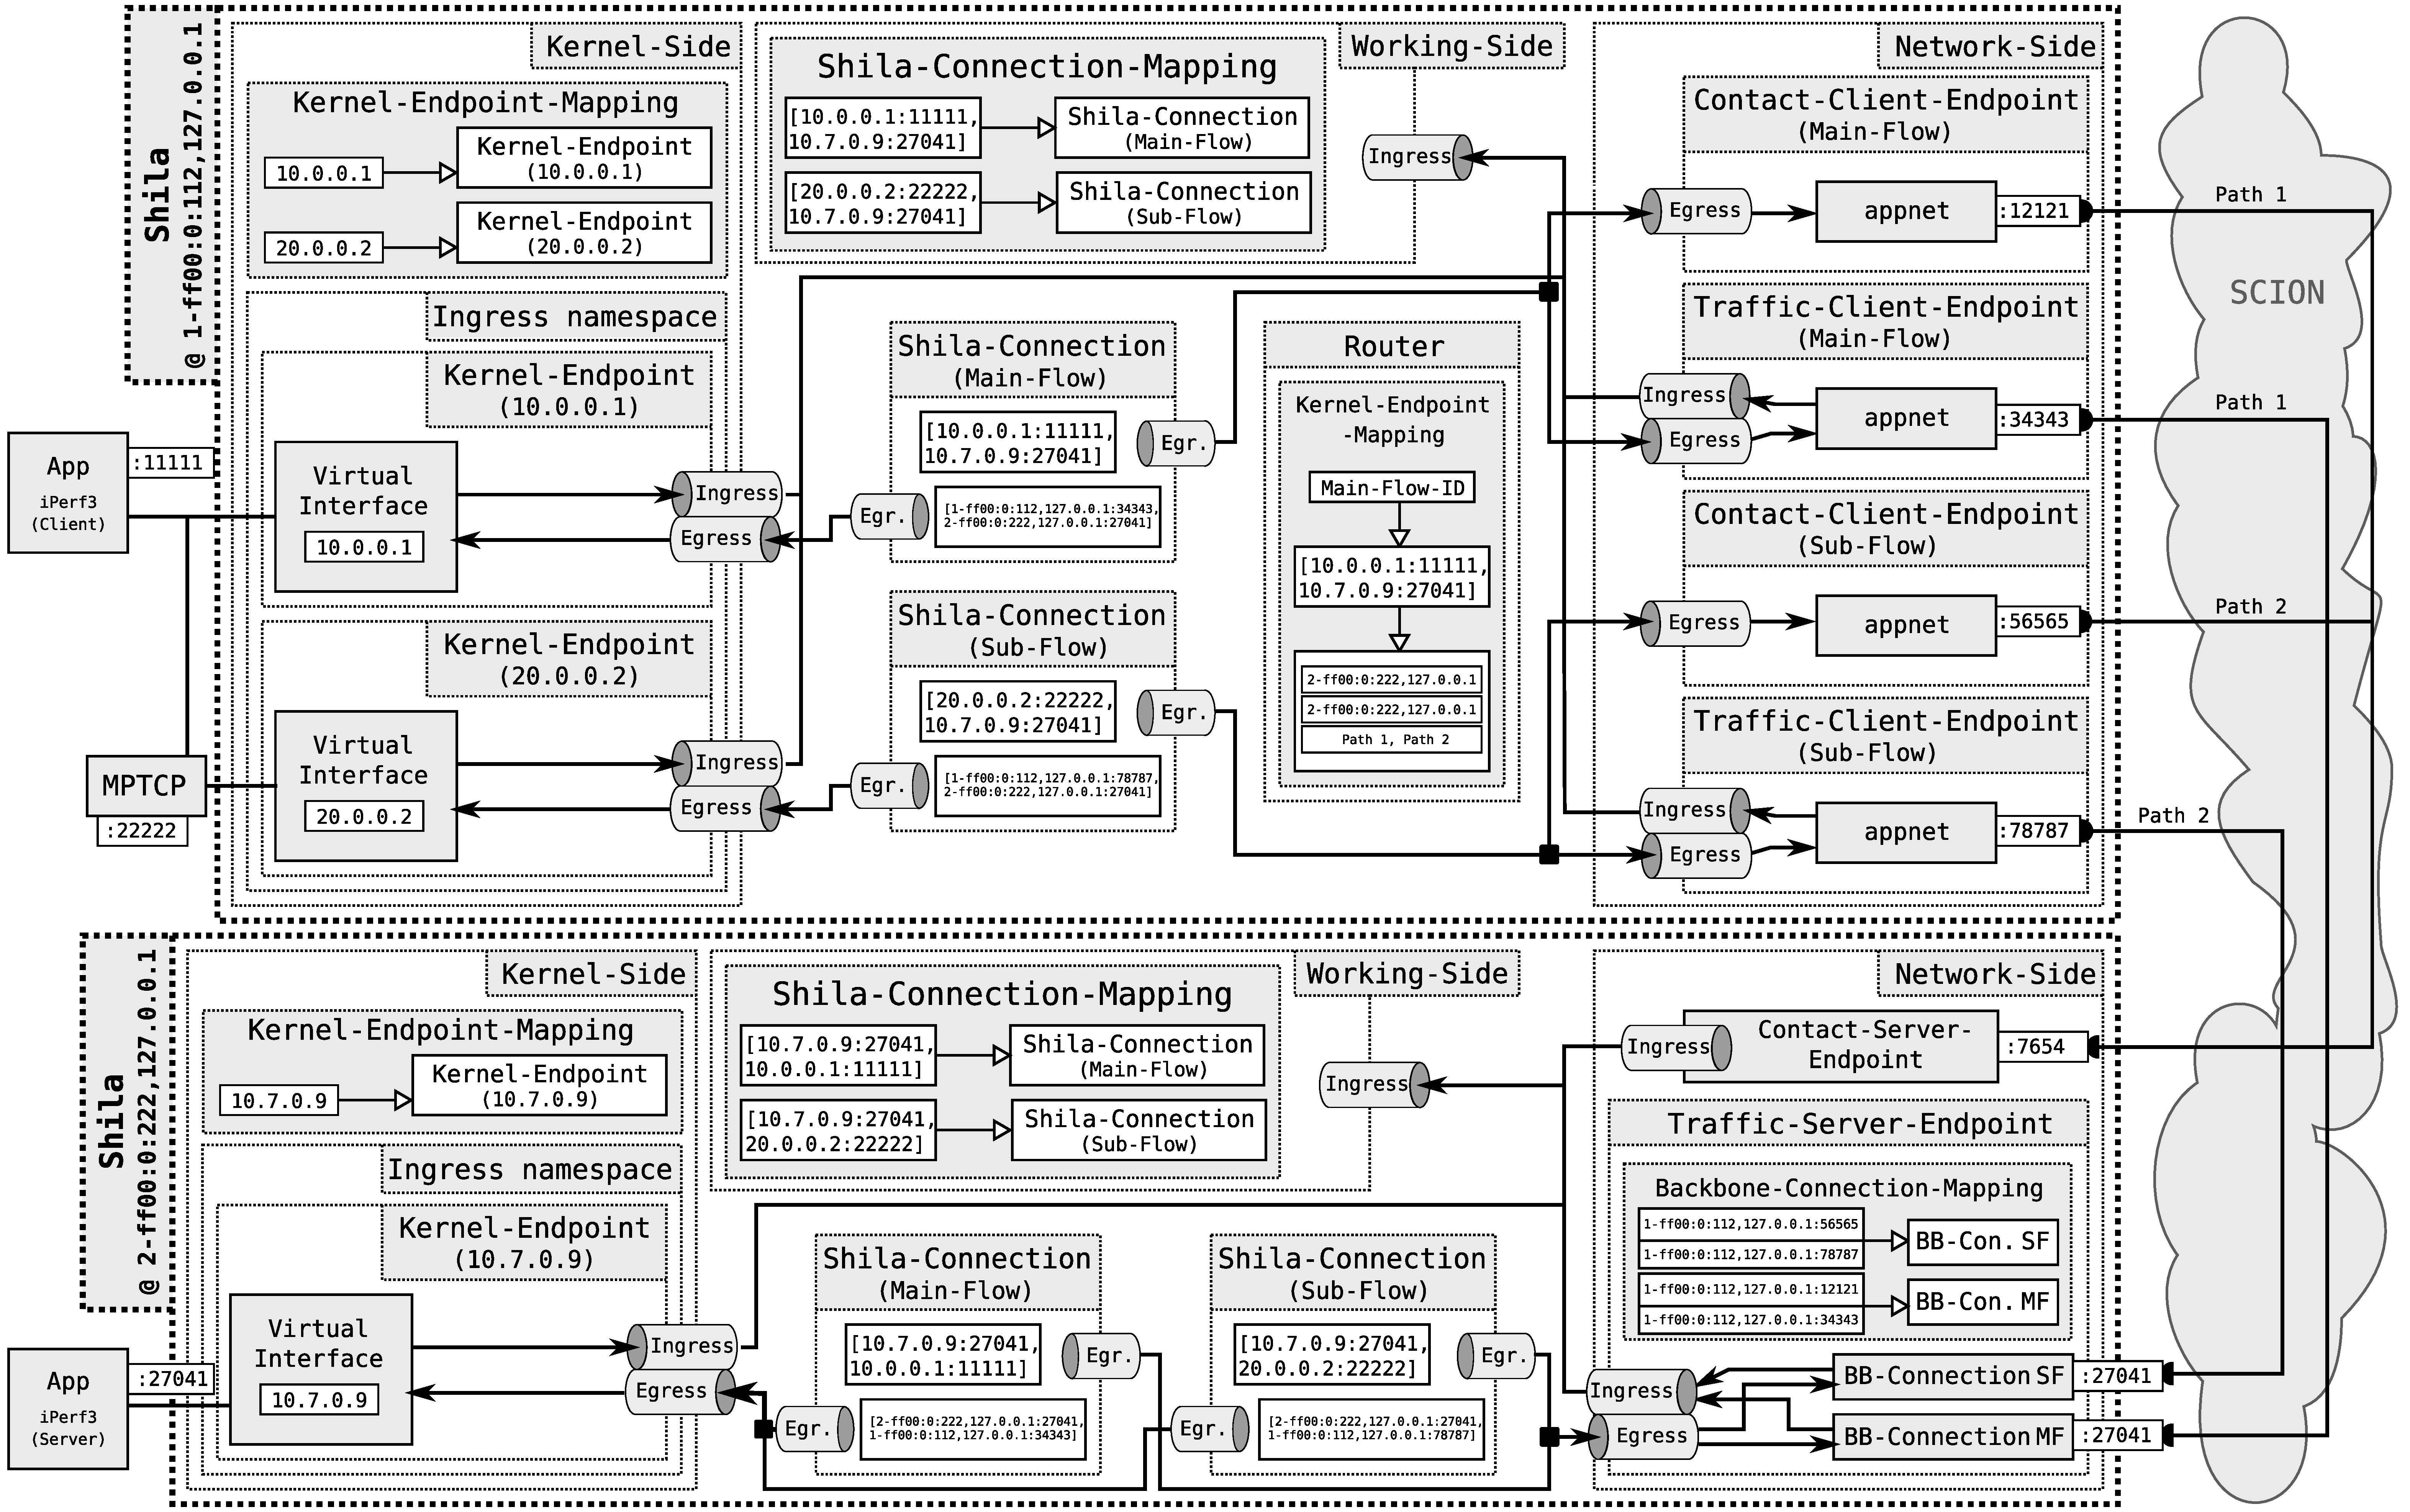
\includegraphics[scale=0.2]{../illustrations/implementation/ConnectionEstablishment.pdf}   
				\caption[Caption for the list of figures.]{Illustration of the State of the Shila instances after the establishment of the Main-Flow and one Sub-Flow. Note that the Contact-Backbone-Connections are removed as soon as the establishment was successful. We show them just for demonstrative purpose.}
				\label{fig:ConnectionEstablishment}
			\end{center}
		\end{figure}
	\end{landscape}
\begin{description}		
	\item[M-15] The IP datagram containing the answer from the iPerf3 server instance, a TCP-SYN+ACK, arrives at the Kernel-Endpoint at Host 2. From there the answer travels in a Shila-Packet, using its TCP-Flow$^{5}$, through the Working-Site to the corresponding Shila-Connection.
	\item[M-16] The Shila-Connection assigns its Net-Flow to the Shila-Packet and forwards it via traffic channel to the corresponding Traffic-Server-Endpoint. From there the TCP-SYN+ACK data finds its way through the Traffic-Backbone-Connection to the corresponding client part. 
	\item[M-17] The reception of the first data from the Traffic-Client-Endpoint on Host 1 concludes the connection establishment. The first response from the Iperf3 Server instance reaches the Shila-Connection, where the Main-Flow-Identifier is extracted. This identifier is used to update the Router accordingly such that Sub-Flows created later can be assigned to their Main-Flow. The response, holding the TCP-SYN+ACK, is then sent along the traffic channel toward the client instance of iPerf3.
	\item[M-18] The Contact-Backbone-Connection is no longer needed and can therefore be removed, together with its corresponding Network-Endpoints.
\end{description}

As soon as the Main-Flow is established, MPTCP starts to initiate further flows, triggering the establishment of Sub-Flows over the other virtual interfaces.

\subsection{Sub-Flow Establishment}

The establishment of Sub-Flow works in the same way as that of a Main-Flow. Therefore, in the following, only the deviating points are mentioned. Of course, the individual entities bind to other ports. But this is not explicitly mentioned and should be clear in illustration \ref{fig:ConnectionEstablishment}.

\begin{description}	
\item[S-2] The initiation for the Sub-Flow is made by MPTCP itself. It binds to one of the yet unused virtual interfaces on Host 1. For our example we assume that port 22222 is chosen. 
\item[S-5] The Router already has an entry, holding destination address and paths. For the establishment of the Sub-Flow, It is sufficient for the Shila-Connection to submit the Main-Flow-Identifier to get the required Net-Flow.
\end{description}

\newpage
\section{Path Selection}
\label{sec:ImplementationPathSelection}

In this section, we discuss the process of determining the Net-Flow given a TCP-Flow or Main-Flow-Identifier. It takes place in the Router and is illustrated as part of Figure \ref{fig:ImplementationShilaConnection}.

During the connection establishment, the Router gets a request from the involved Shila-Connection. It provides either a TCP-Flow if a Main-Flow is about to be established or a Main-Flow-Identifier if a Sub-Flow is about to be established. We start with the explanation of the former and then deal with the latter.

\subsection*{Path Selection in the Main-Flow Establishment}

The Shila-Connection is requesting the Net-Flow for a given TCP-Flow. That is, the Router has to determine and handle the three different entries.

\begin{description}
	\item[Source address] This is the address of the host running the current Shila instance and can be requested from the SCION daemon.
	\item[Destination address] The Router first extracts the destination TCP address from the TCP-Flow. Then a request, using the extracted address as key, is placed into the Routing-Information to fetch the corresponding SCION destination address.
	\item[Path] By querying the SCION daemon the Router receives a set of possible paths leading to the previously fetched destination address. From this collection, the Router selects the best possible subset and stores it together with the SCION destination address in a Shila-Routing-Entry. The Routing-Mapping is accordingly updated with the TCP-Flow and the Main-Flow-Identifier such that the entry is later found when needed in the routing for a Sub-Flow establishment. Finally, the best path from the extracted subset is selected for the Net-Flow.
\end{description}

It remains to be clarified by which criteria the Router determines the best subset of paths. Its cardinality corresponds to the number of virtual egress interfaces. For a single connection, each interface corresponds to a possible flow for which a path is required. As quality criteria, three different metrics are available: Maximum Transmission Unit (MTU), path length and Sharability \cite{Sharability}. Sharability counts how many times each path segment occurs in a set of paths. It is a measure of the path distinctness. Which metric to use, is decided by the user when starting up Shila. The first two metrics, MTU and path length, are provided directly by the SCION daemon, the router just has to sort the selection of paths accordingly and select the topmost ones. For MTU, the sorting is done in descending order, whereas for the path length in ascending. For Sharability, the Router has to determine the minimizing subset which is computationally expensive. We, therefore, approximate the solution with a greedy approach.

\subsection*{Path Selection in the Sub-Flow Establishment}

The Router gets a Main-Flow-Identifier in the case where the Shila-Connection is about to establish a Sub-Flow. In this case, a Main-Flow has already been created and a corresponding entry exists in the Routing-Mapping. The Router receives the corresponding TCP-Flow through the Main-Flow-Identifier and thus also the Shila-Routing-Entry. It is easy to compile the Net-Flow, all required entries are either easily determined (source address) or are already stored in the entry (destination address, path). For the path, the next best-unused one is taken from the subset of flows stored in the fetched routing entry.

\section{Normal Operation and Clean Up}
\label{sec:ImplementationNormalOperationAndCleanUp}

Once a connection has been established, all the data exchanged between two TCP endpoints flows through the Shila-Connections and Backbone-Traffic-Connections of the involved flows. For each IP datagram traveling with MPTCP over SCION, there are either two or three lookups within the participating Shila instances required. The lookup in the Shila-Connection-Mapping is inevitable on both endpoints. If the datagram travels from server to client an additional one in the Backbone-Connection-Mapping is necessary. Also always necessary is the parsing of the IP datagram after its retrieval from the virtual interface, required for the determination of the TCP-Flow. Other than that, the processed Shila-Packet can pass the Shila instances without much interaction. Every Shila-Connection is able to relay the packets directly between the Shila-Endpoints using the handles of the respective traffic channels.

As mentioned in the introductory section, Shila has no influence on which flow of the connection the data uses. This is determined by MPTCP and depends among others on the choice of the congestion algorithm or the scheduler. It is generally not possible for Shila to interact with an established connection, it mainly acts as a relay station.

Shila maintains an established connection as long as there is data flowing. If there is no data exchange observable for a certain amount of time, then the connection is terminated. Meaning that the Traffic-Backbone-Connections is closed and the associated infrastructure is removed. Optimally, the time out value for removing a connection is greater than the keepalive time \cite{KeepaliveWiki} of the TCP connection.

\section{Remark}

In addition to a structure that is as modular as possible and a clear separation of the individual functionalities, the completion of a functional version of Shila had high priority within this work. Based on such a first working version, measurements could be carried out to evaluate the performance of Shila for the first time. We discuss these performance measurements in the following Chapter \ref{chap:PerformanceEvaluation}. It is also clear that a first implementation always has in some sense prototype character and that the quality and performance can be further improved in further revision cycles. Hence are possible extensions and inputs for future work discussed in Chapter \ref{chap:FutureWork}.